\chapter{Introduction \& Objectives}\label{section:introduction}

Before robots can be deployed in safety-critical environments, we must be able to verify they they will perform safely. In cases where real-world testing is too risky or expensive, robotics engineers must instead rely on mathematical modeling or simulation to verify that a robot will perform as intended. Unfortunately, there are issues with each of these approaches. Although mathematical models are amenable to formal proofs, robots are often too complex to reduce to a set of equations. On the other hand, although simulators can handle the full complexity of a robotic system, they are often treated as black-boxes, providing an incomplete view of a robot's performance. In order to safely deploy complex robots in the real world, we require new tools that blend the rigor of mathematical modeling with the scalability and generality of simulation.

In my thesis, I aim to close the gap between formal methods based on mathematical models~\cite{beltaFormalMethodsControl2019,kress-gazitSynthesisRobotsGuarantees2018} and simulation-based verification techniques~\cite{zhouRoCUSRobotController2021,corsoSurveyAlgorithmsBlackBox2021,okellyScalableEndtoEndAutonomous2018} to develop tools to help engineers more easily \textit{design} and \textit{verify} complex robotic systems. My key insight is that simulators, as computer programs, are not black boxes but instead contain rich mathematical structure. If we can exploit this structure using program analysis tools (e.g. automatic differentiation, tracing, etc.), we can combine the flexibility of simulation with the rigor of mathematical reasoning.
%
Using this insight, I aim to develop tools to support the \textit{design-analysis cycle} for robots and other safety-critical cyberphysical systems in three ways:
\begin{enumerate}
    \item \textit{Design optimization:} automatically search for design parameters that achieve good performance.
    \item \textit{Safety verification:} characterize the robustness of a design and predict corner cases where it is likely to fail (either by violating a constraint or incurring a high cost).
    \item \textit{Verification-guided design:} closing the feedback loop between verification and design, e.g. by using predicted corner cases to guide future design iterations.
\end{enumerate}

These tools will support engineers in developing increasingly complex robotic systems, enabling a more efficient design process and providing the ability to verify the safety of a design \textit{before} deployment. Moreover, I will apply my research not just to traditional robotic systems, but to cyberphysical systems such as large-scale energy, transportation, and industrial networks.

\subsection{Impact}

Recent years have seen large numbers of learning-enabled autonomous systems deployed in the real world. Unfortunately, increased deployment has seen a corresponding increase in accidents involving these systems. More and more, the development and deployment of autonomous systems risks being stalled due to public and regulatory concern over safety~\cite{posadaEA22002Autopilot}. Unlike other forms of safety-critical infrastructure like bridges and buildings, autonomous systems suffer from both \textit{complexity}, leading to difficult-to-predict emergent behavior resulting from interactions between subsystems, and \textit{uncertainty} stemming from the environment or the actions of other agents. While engineers in other fields have access to a range of computer-aided tools to boost their productivity and ensure the safety of their designs, such as computer-aided design (CAD) and finite-element analysis (FEA) in mechanical and civil engineering or electronic design automation (EDA) in electrical engineering, robotics engineers lack such comprehensive design and verification tools. In the abscence of these tools, engineers must rely on an ad-hoc process relying heavily on experience and tedious parameter tuning. In my thesis, I aim to address this gap by developing efficient computational tools to assist engineers in designing and verifying safety-critical autonomous systems, with the goal of helping engineers more confidently \textit{design}, \textit{debug}, and \textit{deploy} autonomous systems.

\subsection{Outline}

% TODO update this
% The rest of this document is structured as follows. Section~\ref{section:lit_review} provides the necessary background and reviews related work with an eye towards highlighting the significance of my proposed thesis contributions. Section~\ref{section:local_methods} presents progress that I have already made towards my thesis objectives by designing methods that solve verification-guided design problems using local optimization with gradients derived from differentiable simulation. These methods demonstrate good performance on a range of robotics and control problems, but they rely on local methods that do not give a complete picture of system safety. Section~\ref{section:global_methods} presents in-progress work that addresses this issue by using approximate Bayesian inference rather than optimization, which allows for more exploration of the design/failure search spaces and are more robust to inaccuracies in automatically-computed gradients.

% As robots have become more capable, they have become more complex. Even relatively simple robots will usually several interacting subsystems (e.g. perception, localization, planning, control, etc.) and a large number of sensors and actuators. Adding to this complexity, some subsystems may be model-based, while others might be learned (and thus harder to debug manually).  The result is that the design space for robot systems is large, and the performance of the system is highly sensitive not only to the design choices made in each subsystem but also to potentially uncertain interactions with the environment.

% To design complex systems, engineers in many fields use computer-aided tools to boost their productivity. Mechanical engineers can use a suite of 3D CAD (computer-aided design) and FEA (finite-element analysis) tools to design structures and understand their performance. Likewise, electrical engineers use electronic design automation tools, including hardware description languages like Verilog, to design and analyze large-scale, reliable, and yet highly complex integrated circuits. Sadly, when it comes to designing autonomous systems and robots, there is a lack of these tools, leaving engineers to take an ad-hoc approach relying heavily on experience and tedious parameter tuning.

% In this thesis, I will attempt to address this gap by developing efficient computational tools to assist engineers in designing and verifying safety-critical autonomous systems, with the goal of helping engineers more confidently \textit{design}, \textit{debug}, and \textit{deploy} autonomous systems.

% \subsection{Challenges in designing and verifying of autonomous systems}

% Two factors have made it difficult to develop automated design tools for robotics. The first is \textit{complexity}: most robots are composed of many interacting subsystems. Although some tools may aid in designing certain subsystems (e.g. Simulink for controllers, SolidWorks or CATIA for hardware, custom software for training perception systems), these tools cover only a small part of the overall robotics design problem, which includes sensing, actuation, perception, navigation, control, and decision-making subsystems. In addition to being interconnected, these subsystems often have a large number of parameters that require tuning to achieve good performance (neural network-based perception is an extreme example of this trend). Moreover, since few robotic systems are exactly alike, an effective design tool must allow the user to select an appropriate level of abstraction for the problem at hand. As a result, there is a need for flexible computational tools that can help designers optimize complex robotic systems.

% The second difficulty is \textit{uncertainty}. Robots operate in dynamic environments that cannot be fully specified \textit{a priori}, and nonlinear interactions between the robot and its environment can make this uncertainty difficult to quantify. Nevertheless, we must account for this uncertainty during the design process and ensure that our designs perform robustly. Making matters worse, many autonomous systems are susceptible to rare but catastrophic failures where extremely poor performance can occur in the tails of this uncertainty, and any computational design and verification tool must be able to handle these sorts of rare events.

% To see these challenges in practice, recall the series of accidents involving Tesla's Autopilot system crashing into stopped emergency vehicles, which resulted in 1 death and 15 injuries across 14 incidents between 2020 and 2022~\cite{posadaEA22002Autopilot}. Tesla's Autopilot is a complex system, relying on perception, prediction, planning, and control subsystems. This complexity can make failures such as this difficult to predict a-priori, particularly when failures arise from the interactions between subsystems. For example, this particular Autopilot failure was the result of compounding perception errors (misclassifying emergency vehicles), planning errors (not moving over into an adjacent lane), and control limitations (unable to brake quickly enough to avoid the crash). At the same time, the effects of uncertainty can manifest in changing environmental conditions that might degrade perception accuracy, or unpredictable behavior by nearby agents that makes planning more difficult.

% \subsection{Supporting the design-analysis cycle}

% In this thesis, I aim to develop efficient computational tools to assist engineers in designing and verifying autonomous systems while addressing these challenges of complexity and uncertainty. Before diving into my proposed technical approach, it is worth discussing how these tools can fit into a holistic engineering process.

% A simplified model of an engineering process is shown in Fig.~\ref{intro:fig:process}. This process begins when the engineer uses their domain expertise and creativity to define the problem (including the objective and any constraints), select an appropriate architecture to solve the problem (e.g. choice of subsystems, architecture for any neural networks, etc.), and specifies any free design parameters or known sources of environmental disturbance. With this problem definition in hand, the engineer proceeds in a \textit{design-analysis cycle}, iteratively testing the system and updating their design. 

% \begin{figure}[t!]
%     \centering
%     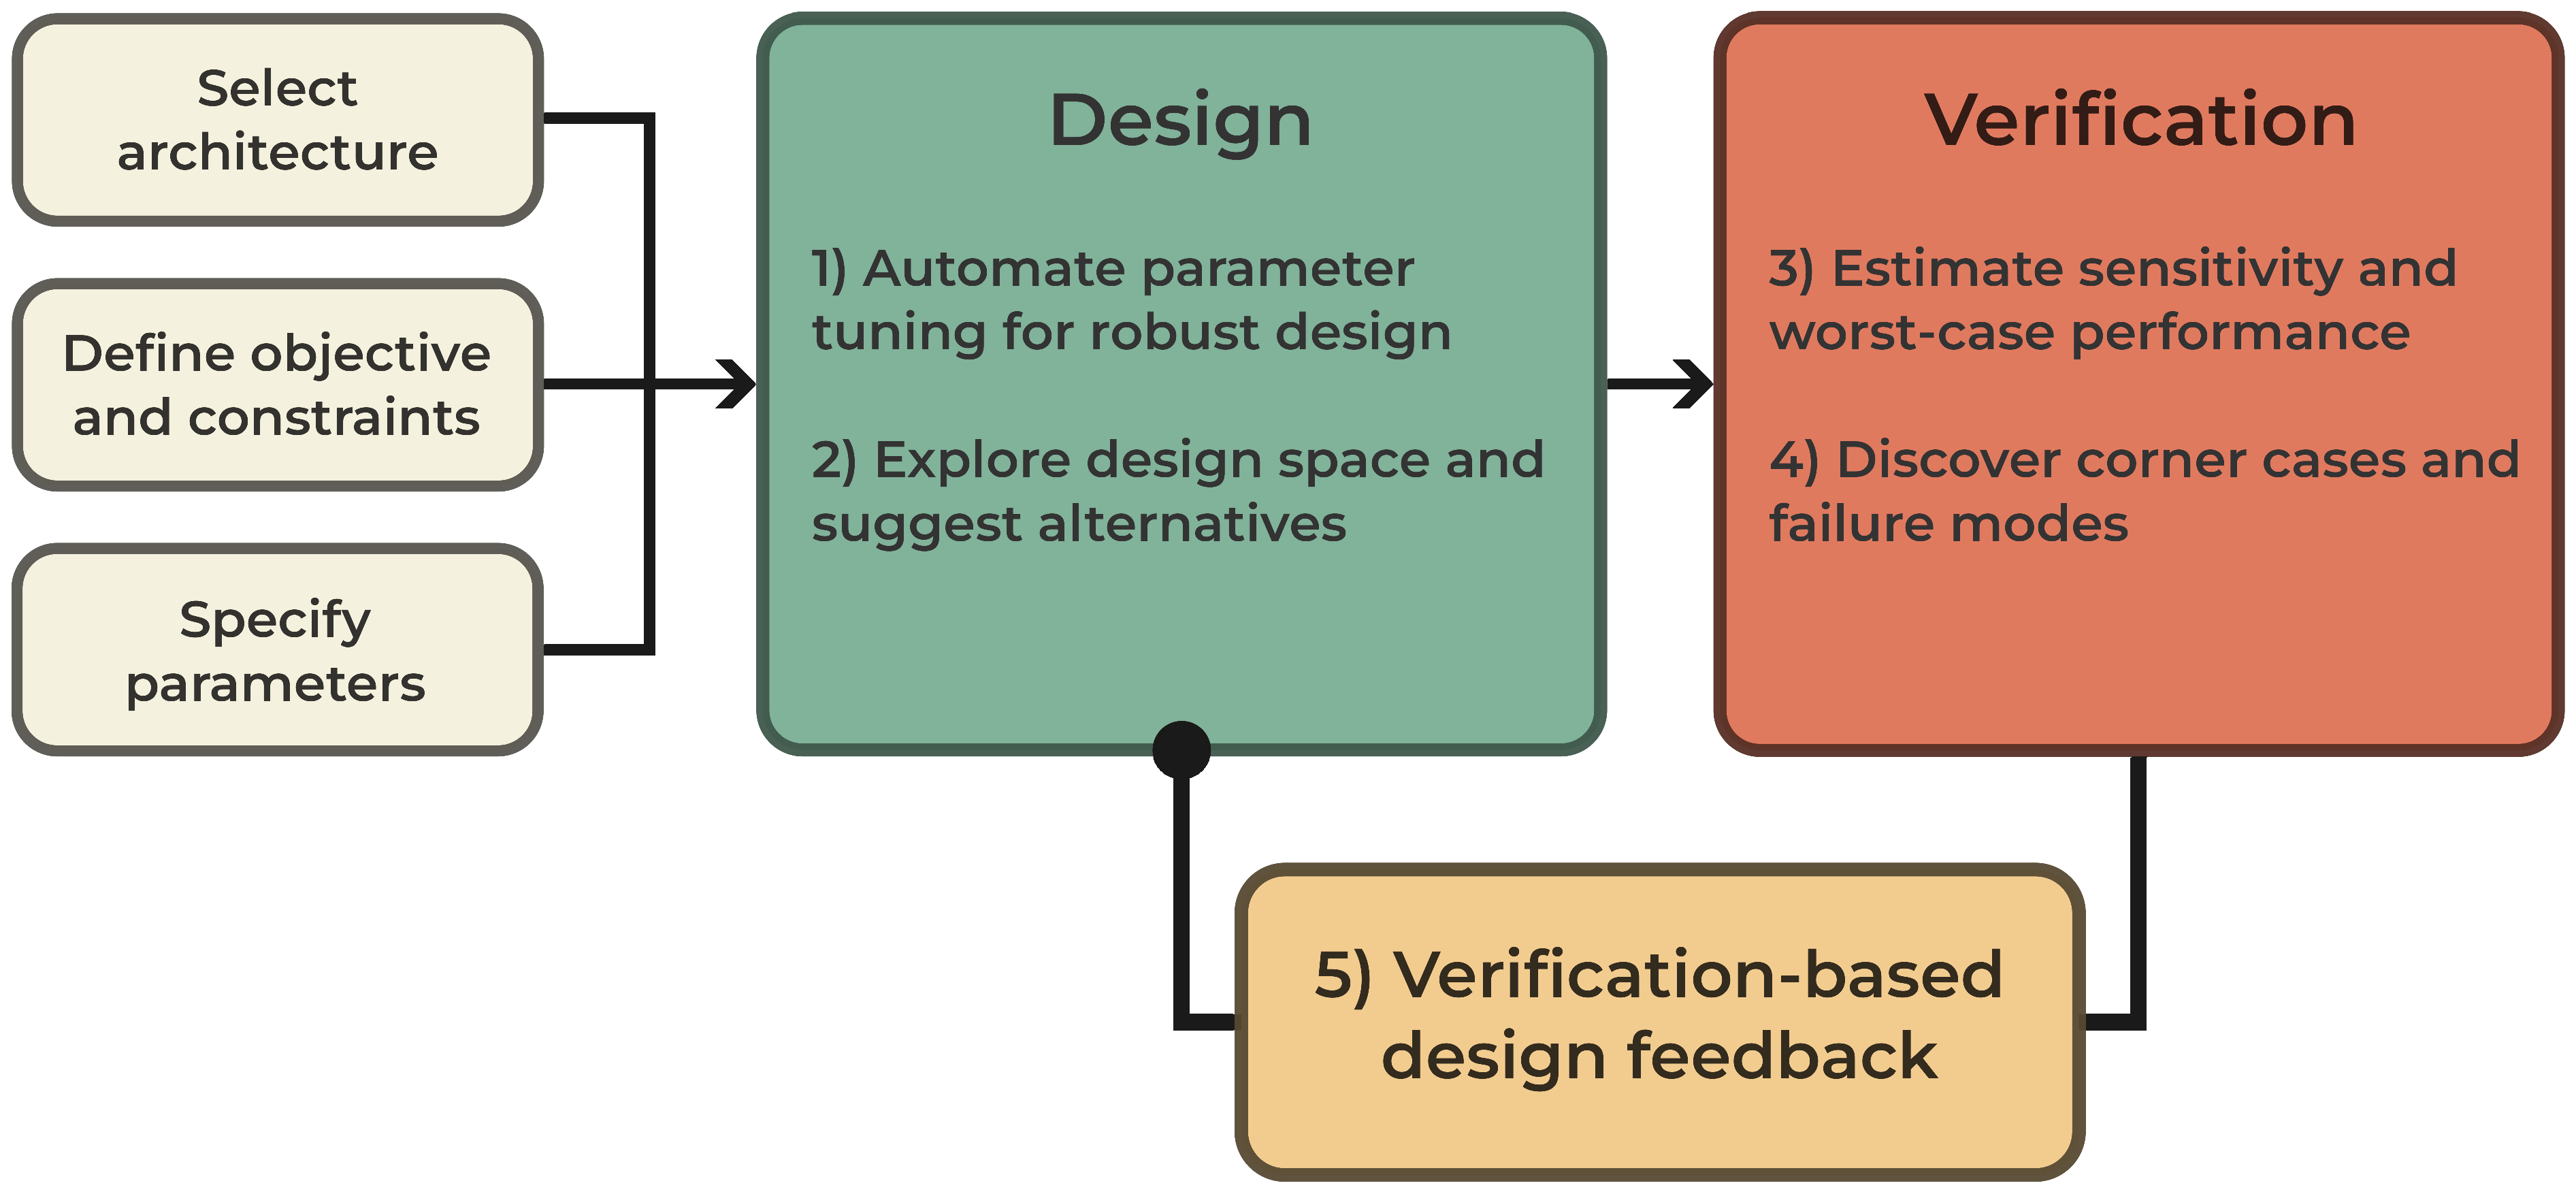
\includegraphics[width=0.7\linewidth]{images/intro/design_process.eps}
%     \caption{A model engineering process, indicating the design and verification stages where my thesis aims to develop computational tools to assist human engineers.}
%     \label{intro:fig:process}
% \end{figure}

% % Zoom in on design-analysis cycle

% % Design tasks: exploring the design space. Fine-tuning designs.

% % Analysis tasks: local adversarial testing, but also exploring diverse failure modes

% % Closing the design/analysis gap: feeding failure modes back into the design process.